\documentclass{article}\usepackage[]{graphicx}\usepackage[]{color}
%% maxwidth is the original width if it is less than linewidth
%% otherwise use linewidth (to make sure the graphics do not exceed the margin)
\makeatletter
\def\maxwidth{ %
  \ifdim\Gin@nat@width>\linewidth
    \linewidth
  \else
    \Gin@nat@width
  \fi
}
\makeatother

\definecolor{fgcolor}{rgb}{0.345, 0.345, 0.345}
\newcommand{\hlnum}[1]{\textcolor[rgb]{0.686,0.059,0.569}{#1}}%
\newcommand{\hlstr}[1]{\textcolor[rgb]{0.192,0.494,0.8}{#1}}%
\newcommand{\hlcom}[1]{\textcolor[rgb]{0.678,0.584,0.686}{\textit{#1}}}%
\newcommand{\hlopt}[1]{\textcolor[rgb]{0,0,0}{#1}}%
\newcommand{\hlstd}[1]{\textcolor[rgb]{0.345,0.345,0.345}{#1}}%
\newcommand{\hlkwa}[1]{\textcolor[rgb]{0.161,0.373,0.58}{\textbf{#1}}}%
\newcommand{\hlkwb}[1]{\textcolor[rgb]{0.69,0.353,0.396}{#1}}%
\newcommand{\hlkwc}[1]{\textcolor[rgb]{0.333,0.667,0.333}{#1}}%
\newcommand{\hlkwd}[1]{\textcolor[rgb]{0.737,0.353,0.396}{\textbf{#1}}}%

\usepackage{framed}
\makeatletter
\newenvironment{kframe}{%
 \def\at@end@of@kframe{}%
 \ifinner\ifhmode%
  \def\at@end@of@kframe{\end{minipage}}%
  \begin{minipage}{\columnwidth}%
 \fi\fi%
 \def\FrameCommand##1{\hskip\@totalleftmargin \hskip-\fboxsep
 \colorbox{shadecolor}{##1}\hskip-\fboxsep
     % There is no \\@totalrightmargin, so:
     \hskip-\linewidth \hskip-\@totalleftmargin \hskip\columnwidth}%
 \MakeFramed {\advance\hsize-\width
   \@totalleftmargin\z@ \linewidth\hsize
   \@setminipage}}%
 {\par\unskip\endMakeFramed%
 \at@end@of@kframe}
\makeatother

\definecolor{shadecolor}{rgb}{.97, .97, .97}
\definecolor{messagecolor}{rgb}{0, 0, 0}
\definecolor{warningcolor}{rgb}{1, 0, 1}
\definecolor{errorcolor}{rgb}{1, 0, 0}
\newenvironment{knitrout}{}{} % an empty environment to be redefined in TeX

\usepackage{alltt}
\usepackage{natbib}
\usepackage[unicode=TRUE]{hyperref}
\usepackage{color}
\usepackage{amsmath, amssymb}
\usepackage{bm}
\definecolor{note_fontcolor}{rgb}{0.800781, 0.800781, 0.800781}
\usepackage{geometry}
\geometry{tmargin=1in,bmargin=1in,lmargin=1in,rmargin=1in}







\IfFileExists{upquote.sty}{\usepackage{upquote}}{}
\begin{document} 

\title{STAT 243 Final Project: Adaptive Rejection Sampling Package}
\author{Mengfei Jiang, Ji Wang, Alexander Fredh-Ojala, Zhuangdi Li}
\date{December 16, 2015}

\maketitle

\tableofcontents

\newpage

\section{Description}
The main function \textit{ars} takes 4 inputs, namely (1) target log-concave density 
function, (2) sample size, (3) lower bound and (4) upper bound, and returns a sample 
by Adaptive Rejection Sampling. The lower bound and the upper bound define the support 
for the target density, and it is assumed that the user input the \textbf{analytically correct 
bounds} when defining the density. $-/+ \infty$ are default values respectively.
The function will then draw samples from the target density after validity checks.\\
\\
To test the package, packages to be installed include 
\href{https://cran.r-project.org/web/packages/testthat/index.html}{\textit{testthat}},
\href{https://cran.r-project.org/web/packages/evd/index.html}{\textit{evd}}, 
\href{https://cran.r-project.org/web/packages/PtProcess/index.html}{\textit{PtProcess}}, 
\href{https://cran.r-project.org/web/packages/smoothmest/index.html}{\textit{smoothmest}}, 
\href{https://cran.r-project.org/web/packages/truncdist/index.html}{\textit{truncdist}}, and
\href{https://cran.r-project.org/web/packages/truncnorm/index.html}{\textit{truncnorm}}.\\
\\
The pakcage is located in Mengfei Jiang's Github repository: \url{https://github.com/MengfeiJiang}
named as \textbf{stat243-project}.

\section{Approach}
The general approach is described by the below pseudo-code:\\
\\
Let A be a set of points $x_i, h(x_i), h'(x_i)$. The tangents at these points
define the upper hull $h_u$, the chords define the lower hull $h_l$.\\
\textit{Repeat}\\
Sample $x$ from $s(x)$, the normalized exponential of the upper hull\\
Sample $u$ from a $Unif(0,1)$\\
\indent \textit{if} $u < exp(h_l(x) - h_u(x))$ then accept $x$ (squeezing)\\
\indent \textit{else} perform the rejection test\\
\indent \indent evaluate function value $h$ at x\\
\indent \indent \textit{if} $u < exp(exp(h(x) - h_u(x)))$ \textit{then} accept $x$\\
\indent \indent \textit{else} reject $x$\\
\indent \indent \textit{endif}\\
\indent \indent update upper and lower hull by adding {$x, h(x), h'(x)$} to A\\
\indent \textit{endif}\\
\textit{until} the user required number of points are sampled\\
\\
Descriptions of each function are detailed as follows.
\subsection{Input Validity Check}
\paragraph{Check support boundaries}
Three checks are performed: lower bound is smaller than upper bound, 
density is neither $-/+ \infty$ or smaller than 0 at bounds, and density is not
0 everywhere within the bounds.
\paragraph{Check density convergence}
The function stops when the integral of the unnormalized density diverges within 
the bounds.
\paragraph{Check log-concavity of the density}
Log-concavity check is performed locally at the neighbourhood of each of the 
abscissae, and we require $h_u(x_i)$ be greather than or equal to $h_l(x_i)$. 
The function stops whenever $h_l(x_i)$ exceeds $h_u(x_i)$. The
check is performed as sampling proceeds.

\subsection{Distribution Shape Determination}
\paragraph{Mode finding}
Mode of the target density is to be used to determine the density shape and as
one of the initialization points. R's \textit{optim} function is called
to find such mode.
\paragraph{Shape determination}
We categorize the shape of a distribution into 4 categories, (1) uniform distribution
with constant density within bounds, (2) monotonely decreasing density, (3) monotonely
increasing density, and (4) density mode occurring within bounds. R's built-in
\textit{runif} function is called to generate samples in the first shape category, while
the following steps of ARS are performed to generate samples for the rest of
the categories.

\subsection{Boundary Shrink}
To avoid numerical issues, valid boundaries are shrinked to such an extent that 
the target density is not numerically zero at and within bounds if it is in the 
first place.

\subsection{Initialization}
Initial abscissae are the lower bound, the upper bound, the mode, one point to
the left of the mode and another point to the right of the mode. $h$ value, i.e.
the $log(density)$ value, and $h'$ value is calculated for each of the initial
point.

\subsection{Upper hull and lower hull}
Vectorized auxiliary functions $u$ and $l$ are such that take a vector of $x$'s 
and output the corresponding values at the upper hull and the lower hull. Each time
$h(x)$ is evaluated, the two functions are also updated. Log-concavity check is
performed for all abscissae every time the upper and lower hulls are updated.

\subsection{Intersections of upper hulls}
Intersections of the upper hulls are determined by the following formula:\\
\begin{align*}
z_i &= x_i + \frac{h(x_i) - h(x_{i+1}) + h'(x_{i+1})(x_{i+1} - x_i)}{h'(x_{i+1}) - h'(x_i)}\\
h_u(z_i) &= h'(x_i)(z_i - x_i) + h(x_i)
\end{align*}
, for $i = 1, 2, \dots, n$, and $z_0 = $ lower bound.\\
$z$'s are updated each time the upper hull and the lower hull are updated.

\subsection{Sampling}
\paragraph{CDF}
CDF up to each intersection point is calculated as follows:\\
\begin{align*}
cdf(z_0) &= 0\\
cdf(z_i) &= \frac{1}{constant}\sum_{j = 0}^{i} \frac{1}{h'(x_{j+1})}{exp(h_u(z_{j+1})) - exp(h_u(z_{j}))}
\end{align*}
, for $i = 1, 2, \dots, n$ and 
$$constant = \sum_{j = 0}^{n-1} \frac{1}{h'(x_{j+1})}{exp(h_u(z_{j+1})) - exp(h_u(z_{j}))}$$
\paragraph{Inverse CDF}
To sample from the customized distribution, we need to inverse the cdf. First, 
draw a vector of $Unif(0,1)$ random variables \textbf{\textit{u}}. Then, for each 
$u_j$, we find the largest $z_i$ such that cdf($z_i$) is smaller than $u_j$. Then,
the $x_j$ sampled from $u_j$ is generated as such to form candidate sample
points \textbf{\textit{x}}:\\
\[
x_j = z_i + \frac{1}{h'(x_{i+1})}log \Big[1 + \frac{h'(x_{i+1})*constant*(u_j - cdf(z_i))}{exp(h_u(z_i))} \Big]
\]
, for $i = 0, 1, 2, \dots, n-1$.
\paragraph{Squeeze test and rejection test}
A vector of $Unif(0,1)$ random variables \textbf{\textit{w}} is generated to
perform squeeze test. All the candidate points up to the first rejected point
are accepted and stored in the final result to be returned. Then, rejection test
is performed on the rejected point, which will be added to the final result if 
accepted. The upper hulls and lower hulls are then updated, and log-concavity
check is performed.\\
If the number of accepted points in the result is smaller than the sample size,
go back to the sampling step and sample until enough.

\section{Testing}
Only representative test results of the main function are detailed in the report.
You may run the full test on the package to see more corner cases that we used to
test the main function.
Unit tests are performed while the package is being developed and are not shown here. 
Both log-concave and non-log-concave distributions are used to test the main function: 
in the former case, the test checks that the sampler correctly samples from some 
well-known log-concave distributions, while in the latter,
an error message should be displayed to the user.\\
\subsection{Log-concave Distributions}
The test output comprises of (1) p-value from 
\href{https://en.wikipedia.org/wiki/Kolmogorov\%E2\%80\%93Smirnov_test}{Kolmogorov-Smirnov test}, 
(2) graphical comparison of the empirical density with the true one,
and (3) QQ-plot of the empirical quantiles and the true.\\
\\
Two-sample Kolmogorov-Smirnov test (or KS test) is used to compare a sample from 
a target unnormalized density generated by ARS with one generated by R's built-in 
function, assuming R's built-in function correctly samples from the underlying true
distribution. It checks whether two data samples come from the same distribution. The
test statistic is $D_{n, n'} = sup_x|F_{1,n}(x) - F_{2,n'}(x)|$, where
$F_{1,n}(x)$ and $F_{2,n'}(x)$ are  the empirical distribution functions of the 
first and the second sample respectively. We would accept that ARS correctly samples
from the target distribution if the p-value of the statistic is greater than 0.05.
Note, the test requires a relatively large sample, and 1000 is the sample
size used for testing.

\subsubsection{Normal}
\begin{knitrout}
\definecolor{shadecolor}{rgb}{0.969, 0.969, 0.969}\color{fgcolor}\begin{kframe}
\begin{verbatim}
## [1] "Sampling  1000  points now!"
\end{verbatim}
\end{kframe}
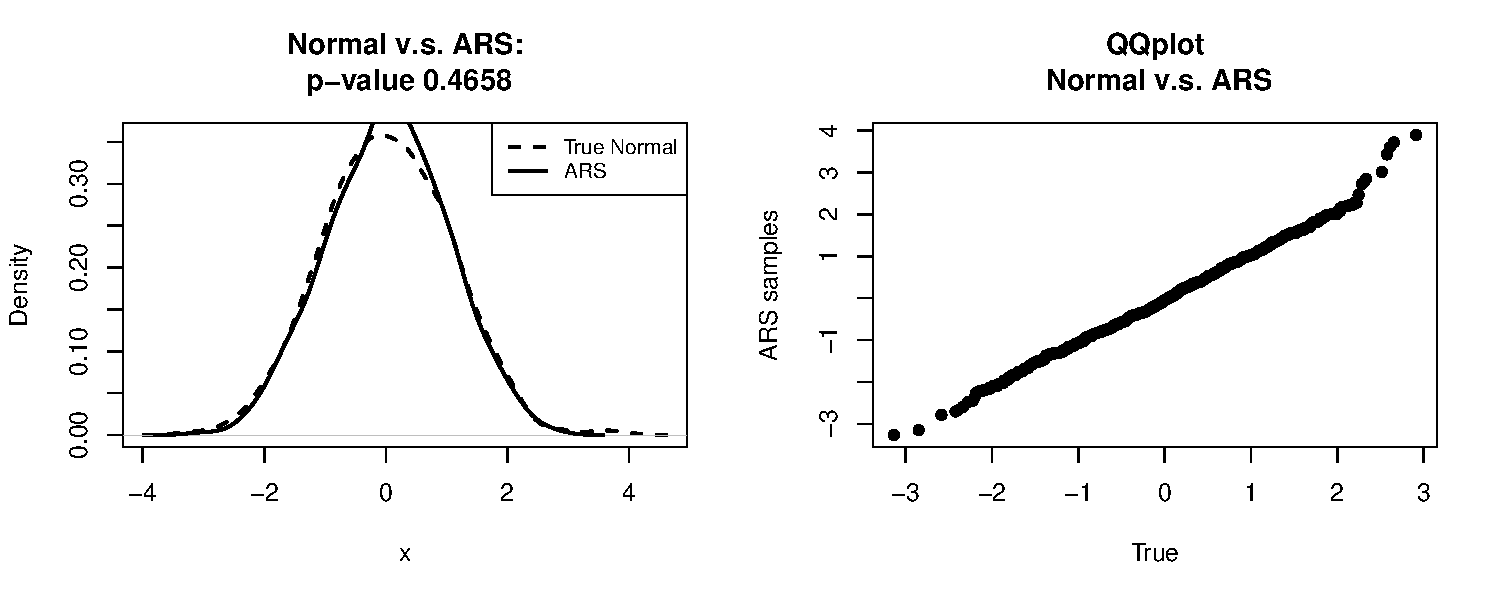
\includegraphics[width=\maxwidth]{figure/normal-1} 

\end{knitrout}

\subsubsection{Truncated Normal}
\begin{knitrout}
\definecolor{shadecolor}{rgb}{0.969, 0.969, 0.969}\color{fgcolor}\begin{kframe}
\begin{verbatim}
## [1] "Sampling  1000  points now!"
\end{verbatim}
\end{kframe}
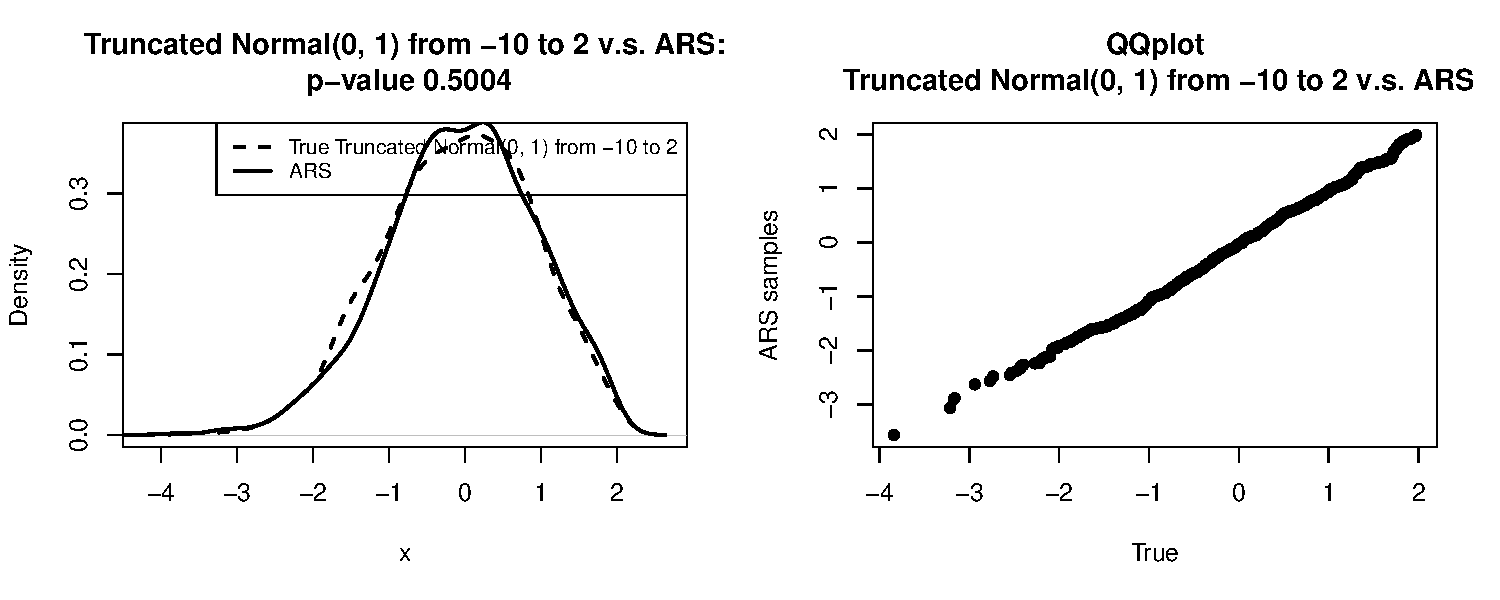
\includegraphics[width=\maxwidth]{figure/truncated_normal-1} 

\end{knitrout}

\subsubsection{Uniform}
\begin{knitrout}
\definecolor{shadecolor}{rgb}{0.969, 0.969, 0.969}\color{fgcolor}\begin{kframe}
\begin{verbatim}
## [1] "Sampling  1000  points now!"
## [1] "Uniform distribution: runif is used to generate sample"
\end{verbatim}
\end{kframe}
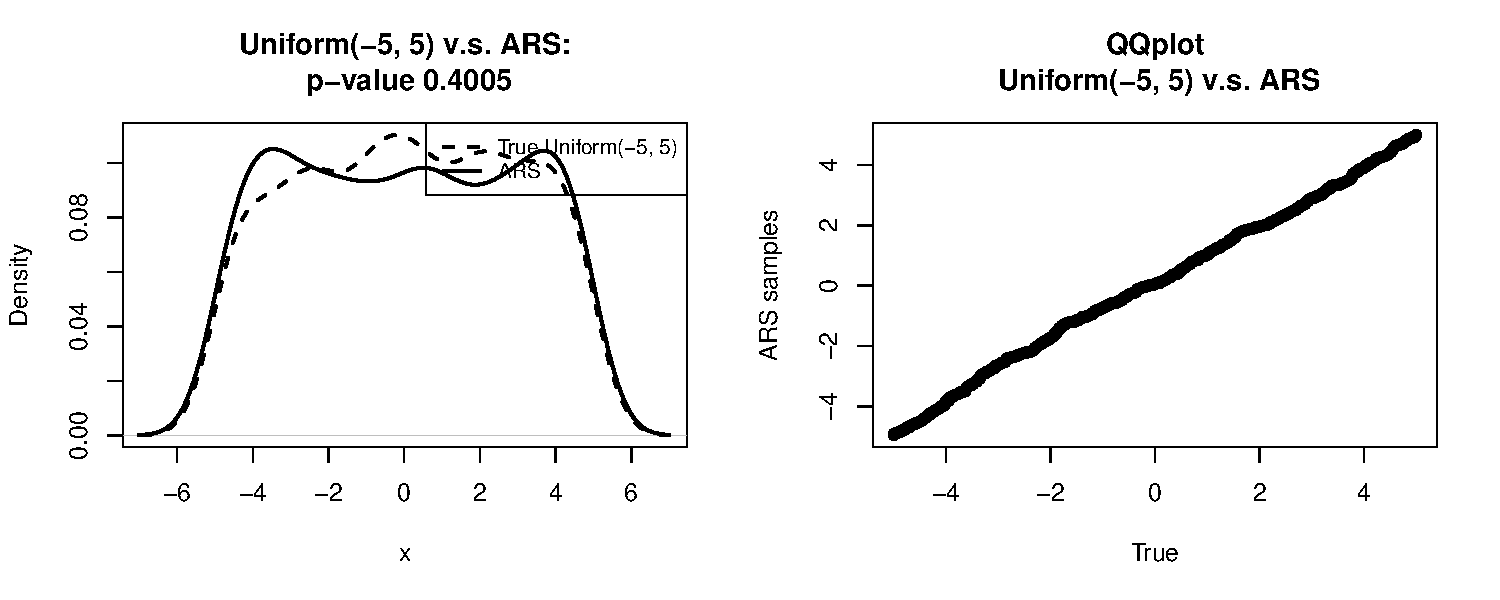
\includegraphics[width=\maxwidth]{figure/uniform-1} 

\end{knitrout}

\subsubsection{Exponential}
\begin{knitrout}
\definecolor{shadecolor}{rgb}{0.969, 0.969, 0.969}\color{fgcolor}\begin{kframe}
\begin{verbatim}
## [1] "Sampling  1000  points now!"
## [1] "Truncated distribution: the leftmost point is the mode."
\end{verbatim}
\end{kframe}
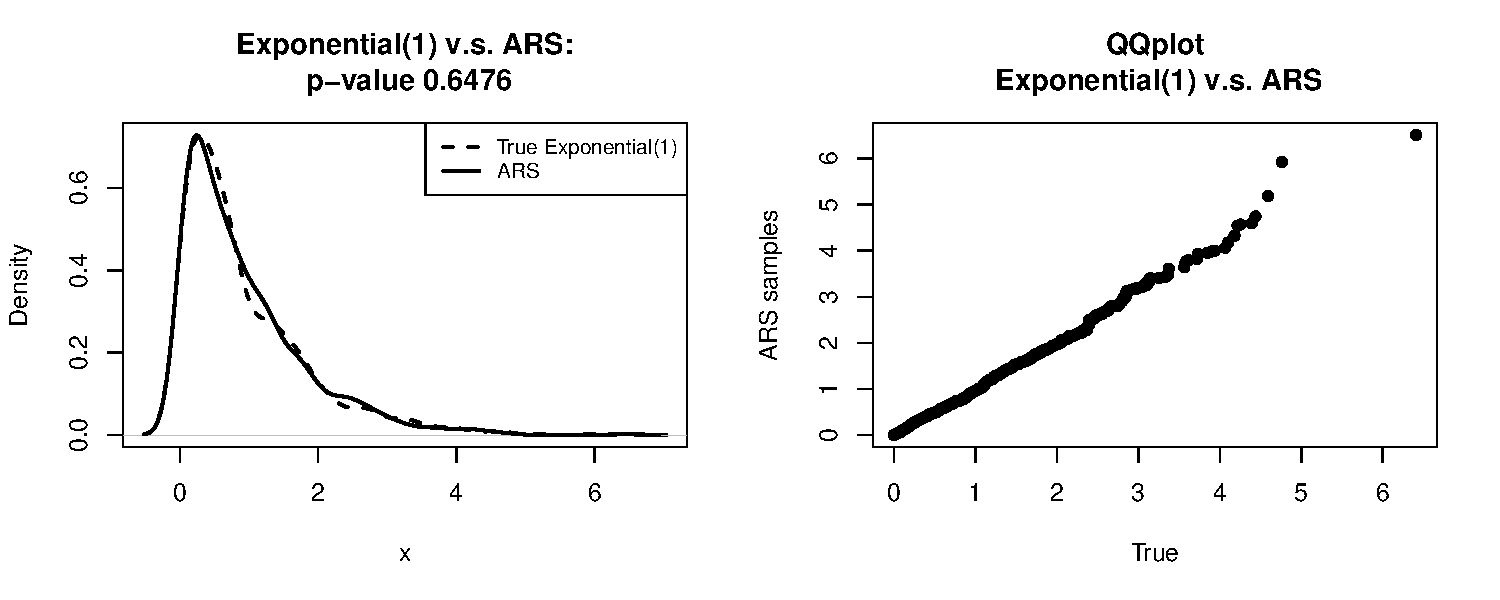
\includegraphics[width=\maxwidth]{figure/exponential-1} 

\end{knitrout}

\subsubsection{Gamma}
\begin{knitrout}
\definecolor{shadecolor}{rgb}{0.969, 0.969, 0.969}\color{fgcolor}\begin{kframe}
\begin{verbatim}
## [1] "Sampling  1000  points now!"
\end{verbatim}
\end{kframe}
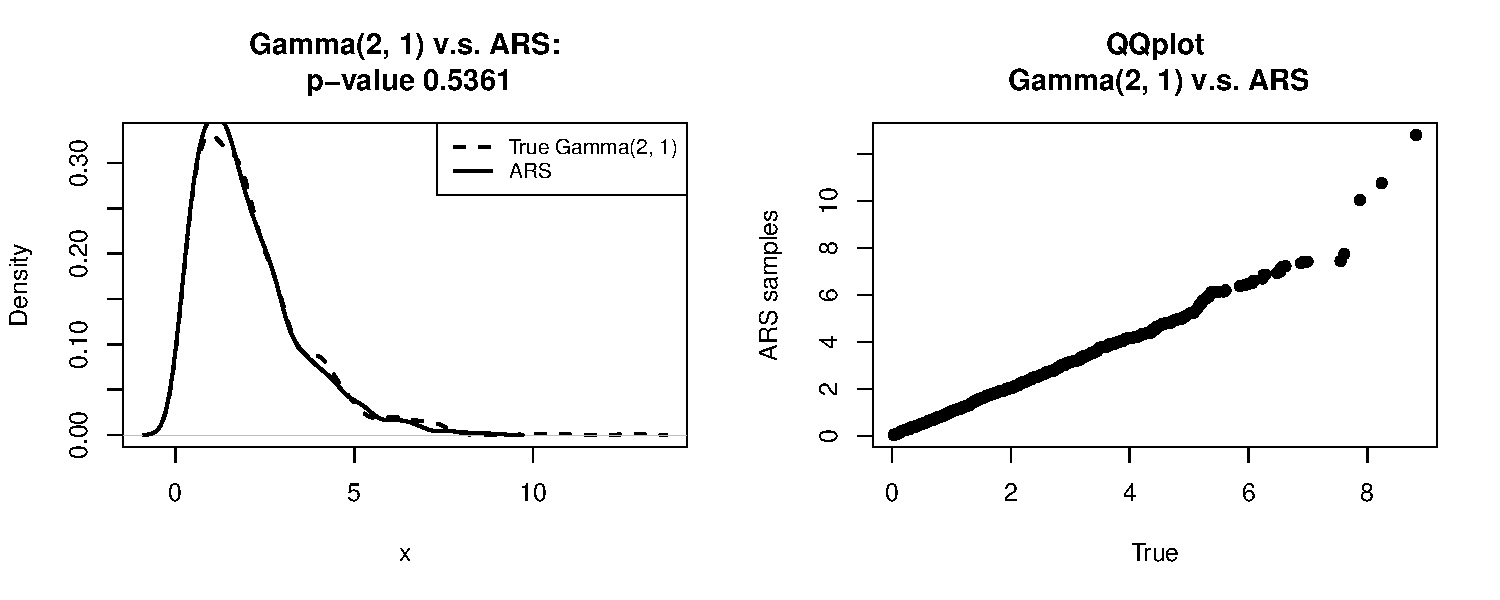
\includegraphics[width=\maxwidth]{figure/gamma-1} 

\end{knitrout}

\subsubsection{Beta}
\begin{knitrout}
\definecolor{shadecolor}{rgb}{0.969, 0.969, 0.969}\color{fgcolor}\begin{kframe}
\begin{verbatim}
## [1] "Sampling  1000  points now!"
\end{verbatim}
\end{kframe}
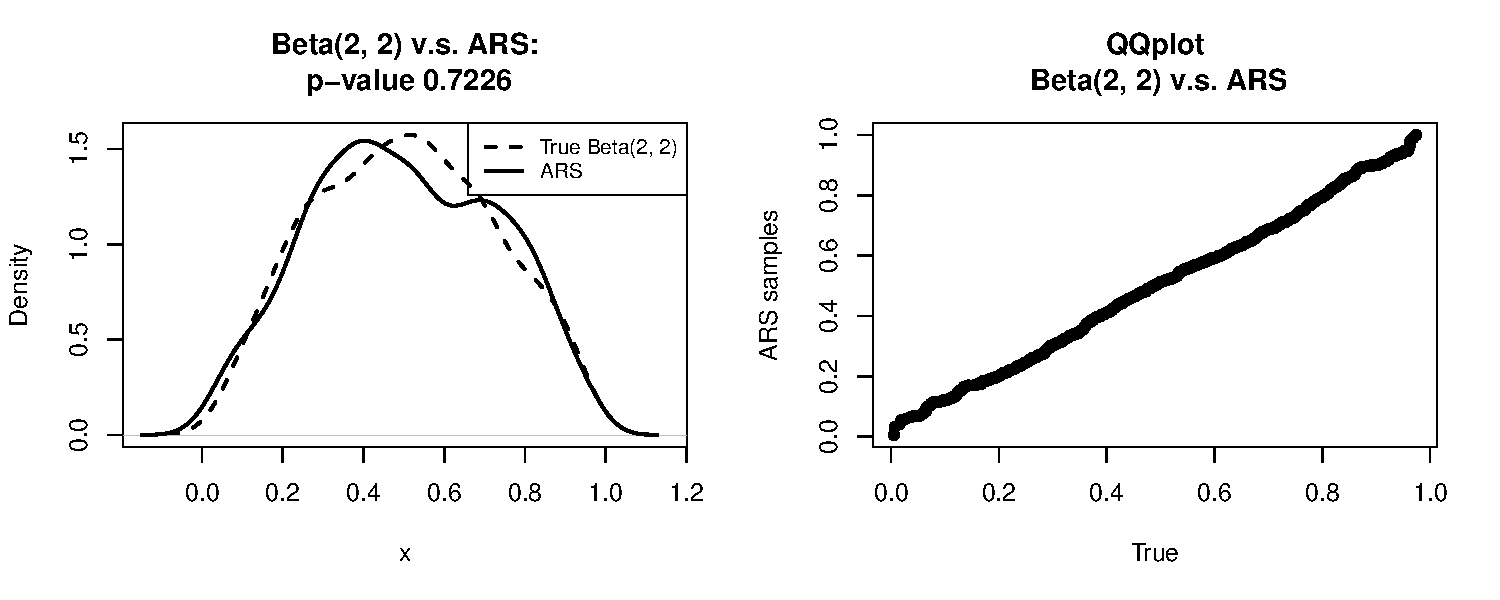
\includegraphics[width=\maxwidth]{figure/beta-1} 

\end{knitrout}

\subsubsection{Logistic Distribution}
\begin{knitrout}
\definecolor{shadecolor}{rgb}{0.969, 0.969, 0.969}\color{fgcolor}\begin{kframe}
\begin{verbatim}
## [1] "Sampling  1000  points now!"
\end{verbatim}
\end{kframe}
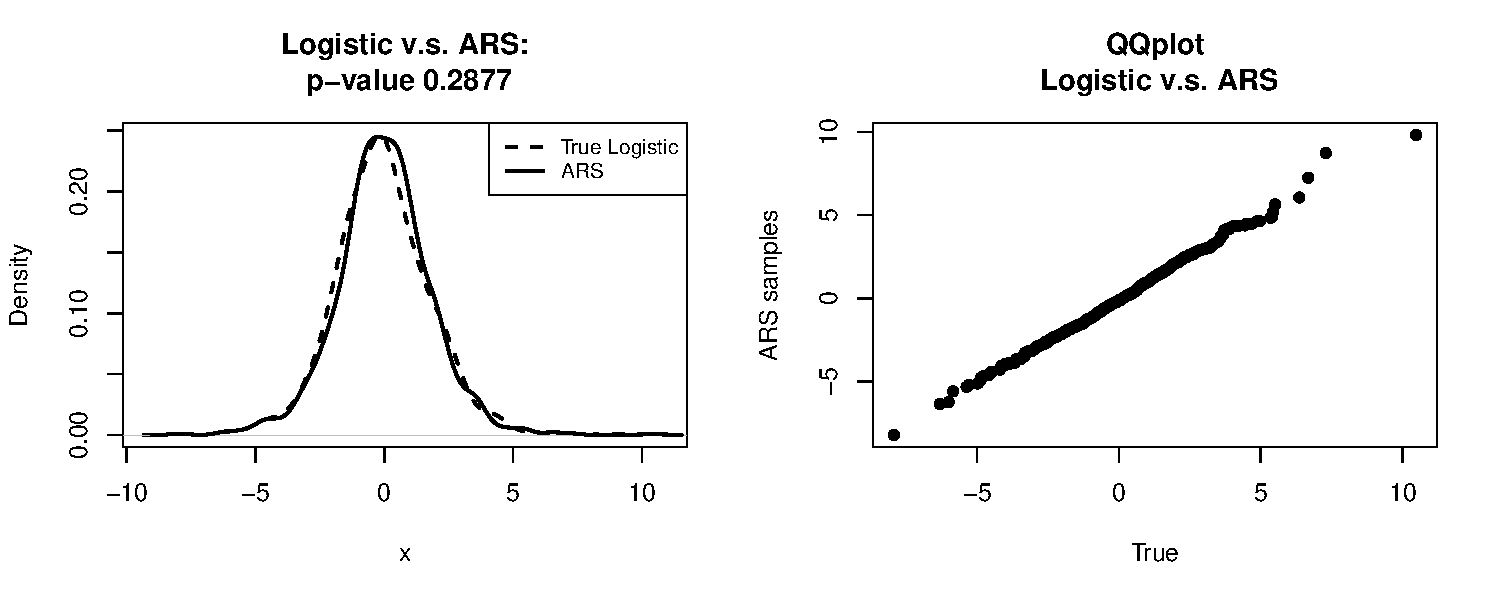
\includegraphics[width=\maxwidth]{figure/logistic-1} 

\end{knitrout}

\subsubsection{Extreme Value Distribution}
\begin{knitrout}
\definecolor{shadecolor}{rgb}{0.969, 0.969, 0.969}\color{fgcolor}\begin{kframe}
\begin{verbatim}
## [1] "Sampling  1000  points now!"
\end{verbatim}
\end{kframe}
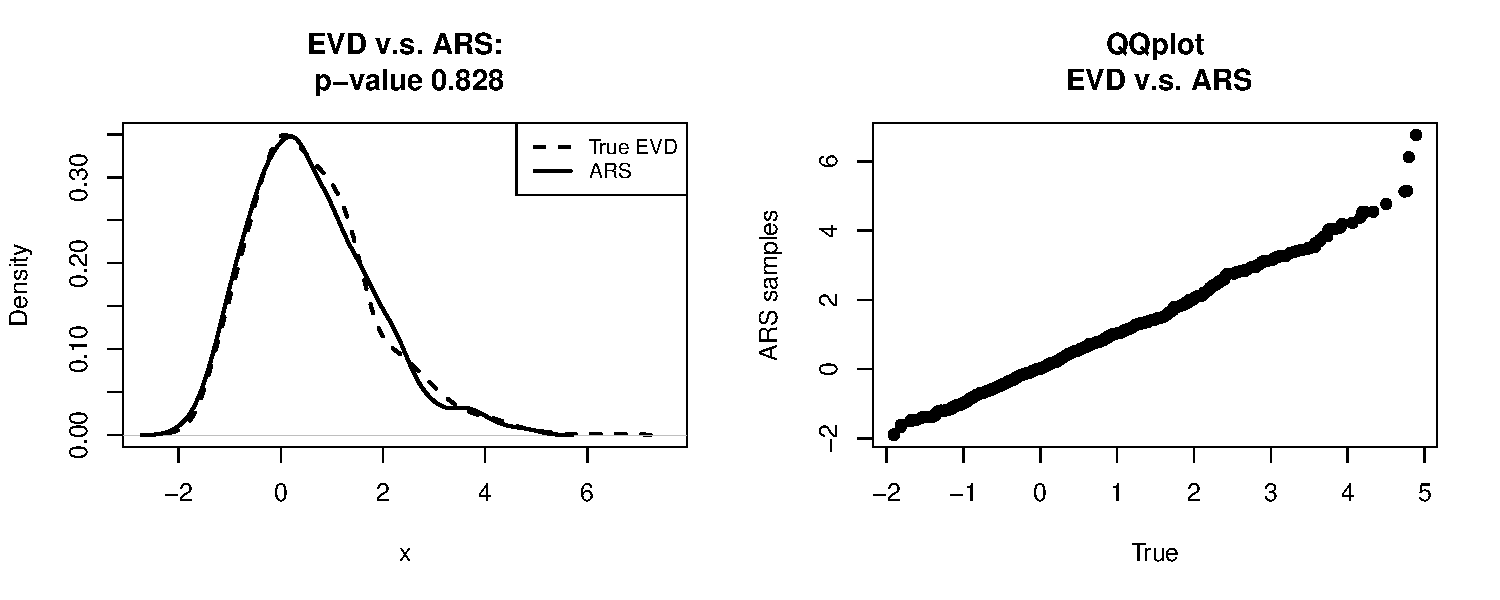
\includegraphics[width=\maxwidth]{figure/extreme_value-1} 

\end{knitrout}

\subsubsection{Laplace}
\begin{knitrout}
\definecolor{shadecolor}{rgb}{0.969, 0.969, 0.969}\color{fgcolor}\begin{kframe}
\begin{verbatim}
## [1] "Sampling  1000  points now!"
\end{verbatim}
\end{kframe}
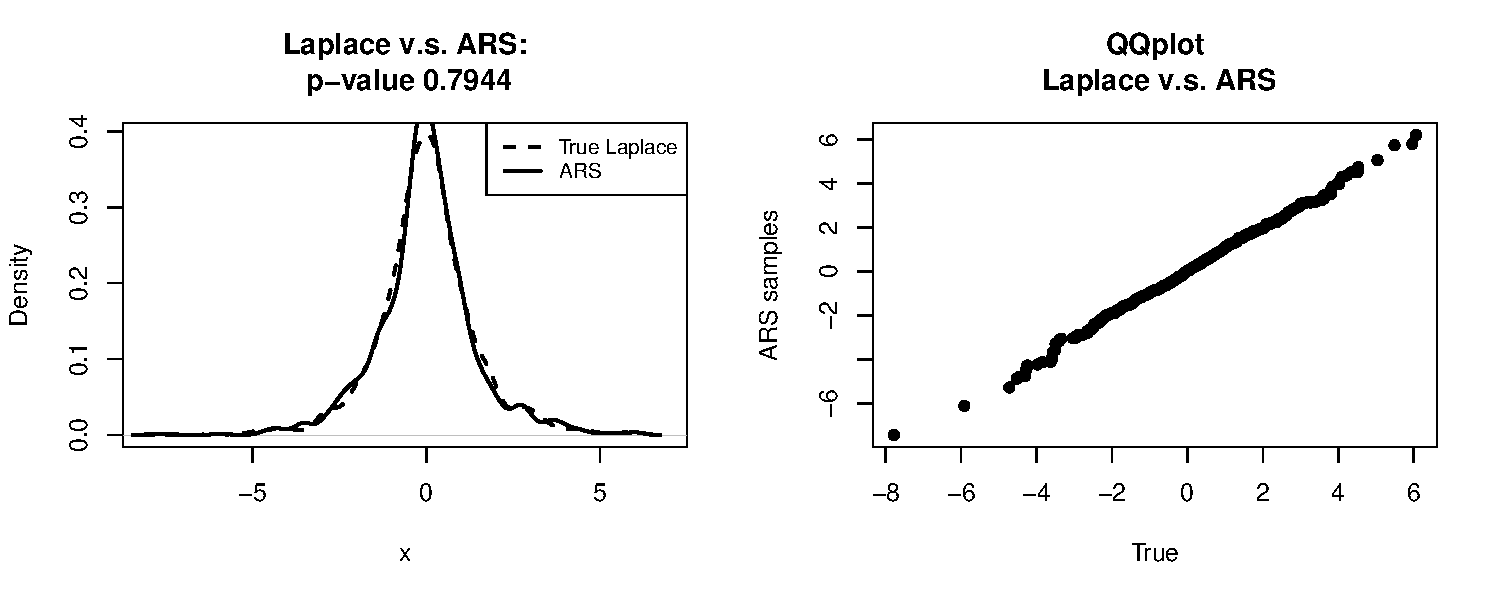
\includegraphics[width=\maxwidth]{figure/laplace-1} 

\end{knitrout}

\subsubsection{Chi-squared with dof $>=$ 2}
\begin{knitrout}
\definecolor{shadecolor}{rgb}{0.969, 0.969, 0.969}\color{fgcolor}\begin{kframe}
\begin{verbatim}
## [1] "Sampling  1000  points now!"
\end{verbatim}
\end{kframe}
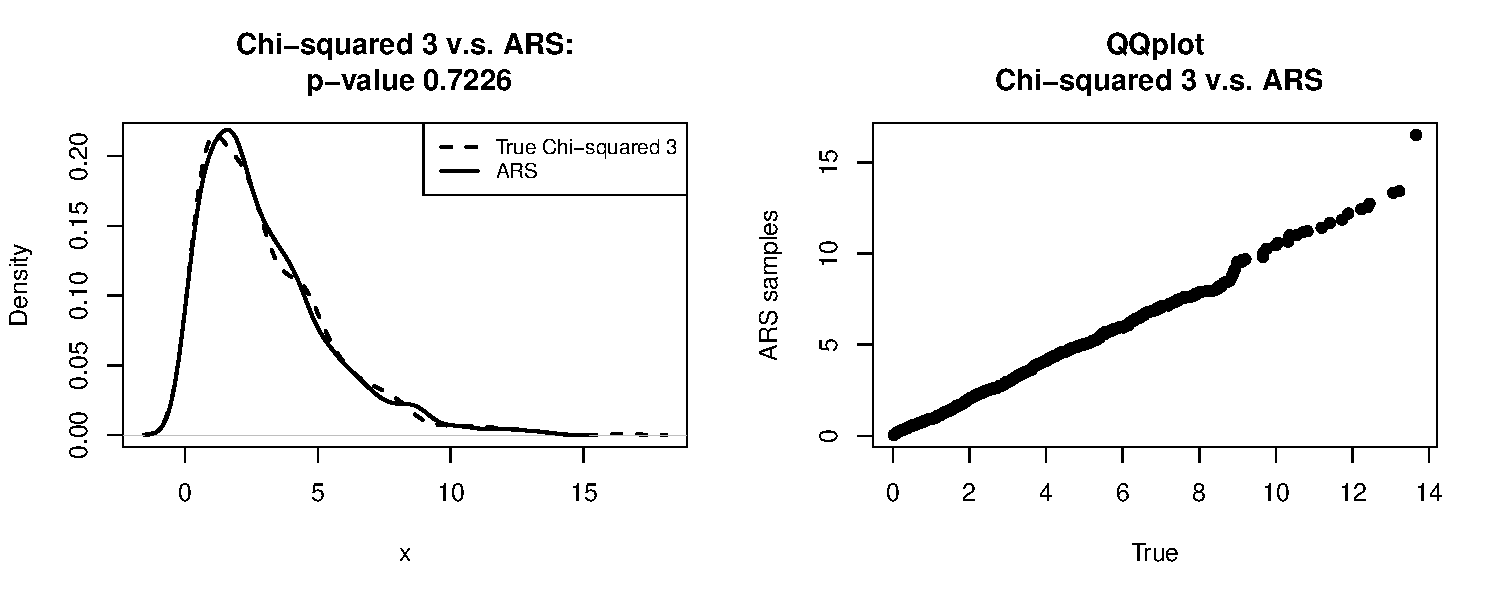
\includegraphics[width=\maxwidth]{figure/chisq_3-1} 

\end{knitrout}

\subsubsection{Weibull Distribution}
\begin{knitrout}
\definecolor{shadecolor}{rgb}{0.969, 0.969, 0.969}\color{fgcolor}\begin{kframe}
\begin{verbatim}
## [1] "Sampling  1000  points now!"
## [1] "Truncated distribution: the leftmost point is the mode."
\end{verbatim}
\end{kframe}
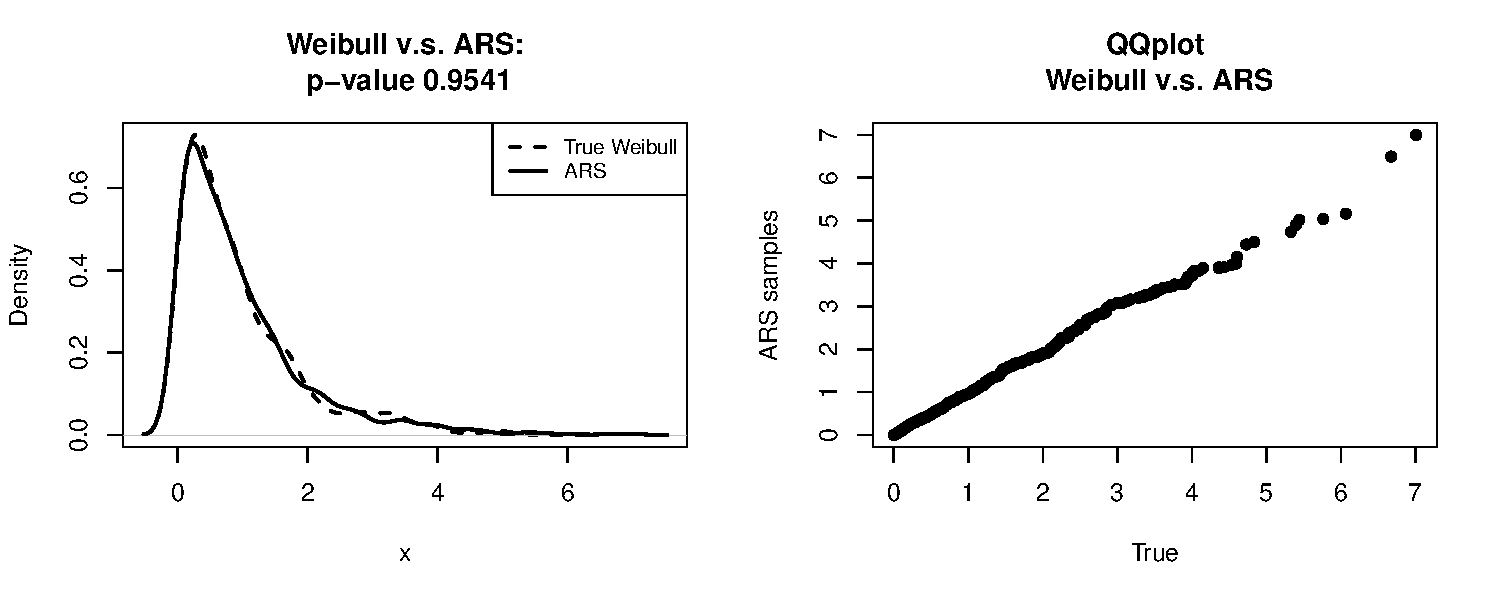
\includegraphics[width=\maxwidth]{figure/weibull-1} 

\end{knitrout}


\subsection{Non Log-concave Distributions}
For the below non-log-concave distributions, it is expected that the sampler
should return an error message about the density not being log-concave and
stops.
\subsubsection{Chi-squared with dof = 1}
\begin{knitrout}
\definecolor{shadecolor}{rgb}{0.969, 0.969, 0.969}\color{fgcolor}\begin{kframe}
\begin{verbatim}
## [1] "Sampling  1000  points now!"
## [1] "Truncated distribution: the leftmost point is the mode."
\end{verbatim}


{\ttfamily\noindent\bfseries\color{errorcolor}{\#\# Error in ars(chisq\_pdf, n, 0.001, Inf): Bad density: not log-concave}}\end{kframe}
\end{knitrout}

\subsubsection{Student's t Distribution}
\begin{knitrout}
\definecolor{shadecolor}{rgb}{0.969, 0.969, 0.969}\color{fgcolor}\begin{kframe}
\begin{verbatim}
## [1] "Sampling  1000  points now!"
\end{verbatim}


{\ttfamily\noindent\bfseries\color{errorcolor}{\#\# Error in ars(t\_pdf, n, -50, 50): Bad density: not log-concave}}\end{kframe}
\end{knitrout}

\subsubsection{Cauchy distribution}
\begin{knitrout}
\definecolor{shadecolor}{rgb}{0.969, 0.969, 0.969}\color{fgcolor}\begin{kframe}
\begin{verbatim}
## [1] "Sampling  1000  points now!"
\end{verbatim}


{\ttfamily\noindent\bfseries\color{errorcolor}{\#\# Error in ars(cauchy\_pdf, n, -Inf, Inf): Bad density: not log-concave}}\end{kframe}
\end{knitrout}

\subsubsection{Pareto Distribution}
\begin{knitrout}
\definecolor{shadecolor}{rgb}{0.969, 0.969, 0.969}\color{fgcolor}\begin{kframe}
\begin{verbatim}
## [1] "Sampling  1000  points now!"
## [1] "Truncated distribution: the leftmost point is the mode."
\end{verbatim}


{\ttfamily\noindent\bfseries\color{errorcolor}{\#\# Error in ars(pareto\_pdf, n, 3, Inf): Bad density: not log-concave}}\end{kframe}
\end{knitrout}

\subsubsection{F-Distribution}
\begin{knitrout}
\definecolor{shadecolor}{rgb}{0.969, 0.969, 0.969}\color{fgcolor}\begin{kframe}
\begin{verbatim}
## [1] "Sampling  1000  points now!"
\end{verbatim}


{\ttfamily\noindent\bfseries\color{errorcolor}{\#\# Error in ars(f\_pdf, n, 1e-05): Bad density: not log-concave}}\end{kframe}
\end{knitrout}


\section{Logistics}
\textbf{Code development}: Mengfei Jiang, Ji Wang, Alexander Fredh-Ojala\\
\textbf{Testing}: Mengfei Jiang, Ji Wang, Alexander Fredh-Ojala, Zhuangdi Li\\
\textbf{Report}: Mengfei Jiang\\
\textbf{Package compilation}: Alexander Fredh-Ojala, Ji Wang\\
\end{document}
